\section{Expérience C4} \label{expC4}
  \subsection{Objectif}
    Comprendre de quelles manières un réseau de neurone connexionniste peut parier sur ses propres résultats
    à partir de ses représentations personnelles.

    
    Réalisation de la seconde expérience de l'article \cite{Cleeremans_2007} sur des données réelles
    non linéairement séparables à l'aide de plusieurs couches dans le perceptron.
  
  
  \subsection{Architecture}
    \paragraph{Description}
      Un premier réseau de perceptron multicouche apprend à discrétiser des fleurs caractérisées
      par 4 neurones d'entrées qui représentent taille et largeur de la pétale et la sépale. 
      Il est composé de plusieurs couche cachée de 5 neurones.
      
      Un second réseau de perceptron multicouche apprend à parier sur la qualité de la réponse
      du premier réseau à partir de ses couche cachées et de sa couche d'entrée.
      
      L'apprentissage du second réseau, n'affecte pas le premier réseau.
    \paragraph{Schéma}
      \begin{center}
	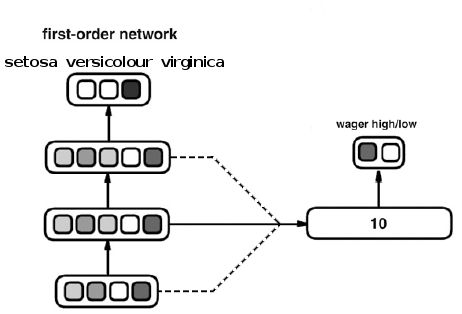
\includegraphics[width=220px]{data/expC4/schema.png}
      \end{center}
      
    \paragraph{Paramètres}
      \begin{center}
	\begin{tabular}{lr}
	  \begin{minipage}{230px}
	    \begin{itemize}
	      \item momentum : 0.9 sur les 2 réseaux
	      \item taux d'apprentissage : 0.1 sur les 2 réseaux
	      \item 10 chiffres différents présentés
	      \item apprentissage 10 (formes) x 1000 (époques)
	      \item utilisation de biais
	    \end{itemize}
	  \end{minipage}
	  &
	  \begin{minipage}{230px}
	    \begin{itemize}
	      \item poids initialisés sur [-0.25 ; 0.25]
	      \item taux d'apprentissage constant
	      \item entrées valent 0 ou 1
	      \item sigmoïde à température 1
	    \end{itemize}
	  \end{minipage}
	\end{tabular}
      \end{center}

  
  \newpage
  \subsection{Résultats}
    \paragraph{Principaux}
      Analyse des performances
      \begin{center}
	\begin{tabular}{lr}
	  \hspace*{-1cm}
	  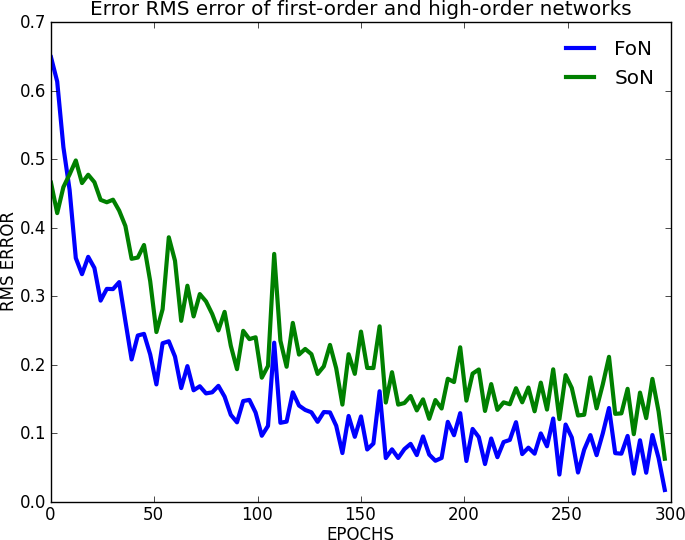
\includegraphics[width=250px]{data/expC4/rms.png}
	  &
	  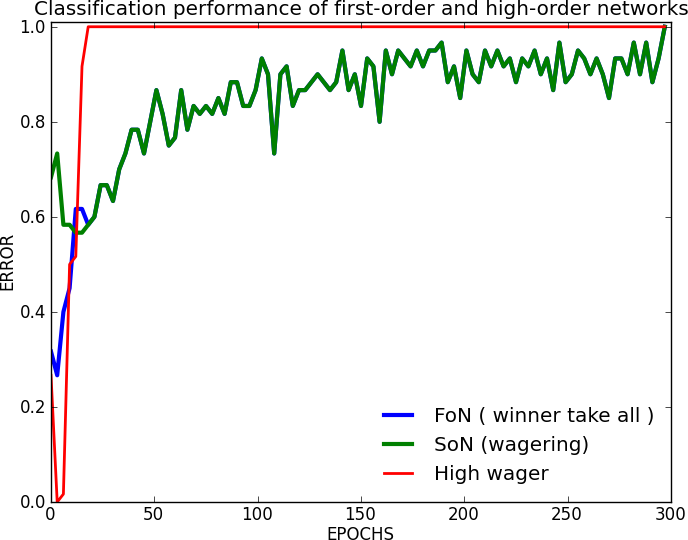
\includegraphics[width=250px]{data/expC4/perf.png} 
	\end{tabular}
      \end{center}
      \subparagraph{Notes}
	\begin{itemize}
	  \item la courbe rouge représentent le taux de paris hauts du second réseau
	  \item la performance de classification représente le taux de bonnes réponses (winner-take-all) pour les 50 formes présentées sur une époque
	\end{itemize}
      \subparagraph{Conclusion}
      Peut importe l'architecture choisi (2 couches cachées, 1 couches cachée, 2 couches cachées + entrées), les performances sont 
      sensiblement les mêmes. 
      
      Le second réseau n'arrive pas à tirer partit des représentations du premier réseau et se contente de partier hauts à chaque fois
      au boût d'un moment.

  \subsection{Conclusion}
    Lors du passage sur des données réelles non linéairement séparables, l'utilité du second réseau
    s'écroule, les représentations ne sont plus exploitées, même avec plusieurs couches.
    
    
    Il faut continuer les essaies pour réussir à le faire fonctionner.	
  

  \newpage 
  \subsection{Formules}
    \paragraph{RMS} \label{rms}
  Pour une époque $e$ :
  \begin{center}
    \begin{large}
    $ rms_{e} = \sqrt{ \frac{1}{n} \sum \limits_{i=1}^{n} 
    ( o_{i,e} - d_{i} )^2 } $
    \end{large}
  $ with \left\lbrace \begin{array}{lll} n : number\ of\ neurons\ on\ the\ output\ 
  layer\\o_{i,e} : value\ obtained\ for\ the\ i^{th}\ neuron\ at\ the\ e^{th}\ epoch\\d_{i} : 
  value\ desired \ for\ the\ i^{th}\ neuron\end{array} \right.$
  \end{center}
    
    \paragraph{Descente de gradient} \cite{Touzet_1992} \\
  Construction de l'erreur : 
    \begin{center}
      $y_{i} = f'(a_i) \times ( d_i - x_i ) \ si\ i\ neurone\ de\ sortie $ \\
      $y_{i} = f'(a_i) \times \sum \limits_{k} ( w_{ki} \times y_k )\ si\ i\ neurone\ cache $
    \end{center}
  Mise à jour des poids :
    \begin{center}
      $w_{ij}(t+1) = w_{ij}(t) + learning\_rate \times y_{i} \times x_j + momentum \times 
      (w_{ij}(t) - w_{ij}(t-1) )$
    \end{center}
  Variables : 
    \begin{center}
      $\left\lbrace \begin{array}{lll} 
	f : fonction\ sigmoide \\
	x_i : valeur\ du\ neurone\ i\\
	d_i : valeur\ desire pour\ le\ neurone\ i\\
	a_i : somme\ pondere\ des\ poids\ du\ neurone\ i
      \end{array} \right.$
    \end{center}
    
\bibliographystyle{../pre-rapport/apalike}
\bibliography{../pre-rapport/biblio}
